\chapter{Ensemble des simulations réalisées}\label{chap:SimusRealisees}
\mylocaltoc

\section{Introduction}
Dans ce chapitre, différents moyens de comprendre les phénomènes prenant place dans le noyau thermoacoustique et dans son voisinage sont expliqués. Tout d'abord, une analyse globale est réalisées dans la section~\ref{chap:NbrAdim} - \nameref{chap:NbrAdim}. Les nombres adimensionnels utilisés dans la littérature pour évaluer la présence de convection naturelle y sont présentés et calculés. Ensuite, un modèle par éléments finis du régime stationnaire est développé dans la section~\ref{chap:FEM} - \nameref{chap:FEM} pour prendre en compte plus de paramètres d'étude. Enfin, un modèle analytique temporel du régime transitoire est présenté dans la section~\ref{chap:ModeleTemporel} - \nameref{chap:ModeleTemporel}.

\section{Modèle simplifié et nombres adimensionnels}\label{chap:NbrAdim}
Au sein du réfrigérateur \textsc{Tacot} et particulièrement dans la cavité devant la source acoustique principale, la distribution de température du côté froid hors du noyau laisse penser à la présence d'une cellule de convection naturelle à l'intérieur. Il est difficile de se rendre compte des flux massique et thermique causés par la différence de température de part et d'autre des différentes zones du \textsc{Tacot} -- volume d'adaptation d'impédance, noyau thermoacoustique -- à cause de leurs géométries, du type de convection naturelle rencontré, de la porosité, etc. Des études hydrodynamiques sont menées pour aider à l'interprétation des mesures de température. \medskip

Tout d'abord, deux étude très simplifiées sont réalisées pour une cavité 2D différentiellement chauffée par des températures chaude $T_c$ et froide $T_f$. Ces études doivent permettre l'obtention d'ordres de grandeurs des quantité d'intérêt, en particulier le flux de chaleur $Q_{conv}$ qui agit comme une charge thermique sur le côté froid du noyau thermoacoustique. \smallskip

Ensuite, des simulations par éléments finis de cette cavité et sur le régénérateur sur le logiciel Comsol Multiphysics permettent d'estimer les lignes de courants dans la cellule et l'influence de cet écoulement sur la distribution de température sur l'échangeur froid, en plus de déterminer des paramètres clés pour la compréhension des phénomènes thermiques en jeu.

\subsection{\'Etudes simplifiées}
\subsubsection{Sans acoustique}
Pour introduire des concepts utiles à la compréhension des phénomènes de convection naturelle, une étude très simplifiée dans une cavité rectangulaire en 2D et représentée sur les figures~\ref{fig:SimuConvNat2D}{\color{MatlabOrange}(a)} et {\color{MatlabOrange}(b)} est menée. 

Dans la première sous-figure~\ref{fig:SimuConvNat2D}{\color{MatlabOrange}(a)}, les parois verticales droite et gauche sont respectivement maintenues à une température froide $T_f$ et chaude $T_c$, tandis que le sol, le plafond et le gaz au repos sont à la température $T_\infty$. En régime stationnaire, il s'établit une cellule de convection naturelle dans laquelle le gaz est mis en mouvement par les  variations de masse volumique proches des parois verticales. Cette configuration s'apparente aux orientations `\texttt{H1}' et `\texttt{H2}', respectivement présentées sur les figures~\ref{fig:OrientationCore_H1} et \subref{fig:OrientationCore_H2}.

Dans la seconde sous-figure~\ref{fig:SimuConvNat2D}{\color{MatlabOrange}(b)}, ce sont cette fois les sol et plafond qui sont fixés aux températures chaude $T_c$ et froide $T_f$, et les murs et le gaz au repos pour lesquels la température est $T_\infty$. Dans cette configuration, favorable a priori à la mise en place d'une instabilité de \og Rayleigh-Bénard \fg{}, il peut s'établir des cellules de convection naturelle de forme plus ou moins complexe au delà du nombre de Rayleigh critique $\Rayleigh_c$ compris entre 650 et 1700 pour des parois à température fixe \cite{getling_rayleigh-benard_1998}. Le gaz s'élève depuis la paroi chaude jusqu'à la paroi froide, de laquelle il redescend ensuite pour revenir à son point de départ. Dans ce cas, la cellule de convection naturelle peut adopter une structure très complexe, plus que ce que peut suggérer la figure~\ref{fig:SimuConvNat2D}{\color{MatlabOrange}(b)} qui ne représente qu'une illustration grossière du mouvement du fluide. Les expériences correspondant à ce cas sont mises en place en suivant les orientations `\texttt{V1}' et `\texttt{V2}', présentés respectivement sur les figures~\ref{fig:OrientationCore_V1} et \subref{fig:OrientationCore_V2}

\begin{figure}[!ht]
    \centering
    \external{fig_SimuConvNat2D}
%    \externalremake
    \begin{tikzpicture}[scale=.95]
	\def\l{5};
	\def\L{7};
	\def\e{.25};
	\def\xdist{9cm};
	\def\ylab{-.75};
		
	% ----------- Flow direction
	\draw[->,dashed,gray,very thick] (-\L/2.5,.5+\l/2) to[out=90,in=90] (\L/2.5,\l/2);
	\draw[->,dashed,gray,very thick] (\L/2.5,-.5+\l/2) to[out=-90,in=-90] (-\L/2.5,\l/2);
	
	% ----------- Rayleigh zone
%	\fill[dotted] (O.center) to[out=0,in=-90] ++(\e)
	
	% ----------- Cavity
	\fill[pattern=north east lines,pattern color=MatlabOrange] (-\L/2,\l) node[above left,color=MatlabOrange]{$T_{c}$} rectangle ++(-\e,-\l);
	\fill[pattern=north east lines,pattern color=MatlabBlue] (\L/2,\l) node[above right,color=MatlabBlue]{$T_{f}$} rectangle ++(\e,-\l);
	\draw[ultra thick] (-\L/2,0) rectangle ++(\L,\l);
	\draw (-\L/4,0) node(O)[above]{$T_{\infty}$};
	
	% ----------- Gravity direction	
	\draw[->,green!50!black] (0,2*\l/3) -- ++(0,-\l/3) node[midway,fill=white]{$\mathbf g$};
	
%	\draw[<->] (-\L/2,\l+.2) -- ++(\L,0) node[midway,above]{$L_c^{(1)}$};	
	
	
	\draw (0,\ylab) node[]{\textbf{(a)}};
	
	% ----------- Zoom sur paroi chaude
	\begin{scope}[xshift=\xdist]
%		\fill[dashed,left color=MatlabOrange!50,right color=white] (0,0) to[out=0,in=-90] node[near start,below right]{$T_\infty$} ++(2,\l) -| (0,0);
%		\draw[<->] (0.1,3*\l/4) -- ++(1.8,0) node[midway,below]{$L_c^{(1)}$};
%		\draw[dotted] (0,3*\l/4) to[out=45,in=135] node(v)[near end]{} ++(2,0) ;
%		\draw[dotted,->] ($(v.north east)+(.75,.5)$) node[right]{\shortstack{Profil\\de vitesse}} to[out=180,in=45] (v.north east) ;
%		\fill[pattern=north east lines,pattern color=MatlabOrange] (0,\l) node[above left,color=MatlabOrange]{$T_{c}$} rectangle ++(-\e,-\l);
%		\draw[ultra thick] (0,0) -- ++(0,\l);
%		
%		
		% ----------- Flow direction
		\foreach \xi in {1,2,3}{
		\node (bottom\xi) at ({\xi*\L/3-\L/6-\L/2},\l/8){};
		\node (top\xi) at ({\xi*\L/3-\L/6-\L/2},{7*\l/8}){};
		\draw[->,dashed,gray,very thick] (bottom\xi.north west) to[out=110,in=-110] (top\xi.south west);
		\draw[->,dashed,gray,very thick] (top\xi.south east) to[out=-70,in=70] (bottom\xi.north east);
		}
		
		% ----------- Cavity
		\fill[pattern=north east lines,pattern color=MatlabOrange] (-\L/2,0) rectangle ++(\L,-\e) node[right,color=MatlabOrange]{$T_{c}$};
		\fill[pattern=north east lines,pattern color=MatlabBlue] (-\L/2,\l) rectangle ++(\L,+\e) node[right,color=MatlabBlue]{$T_{f}$};
		\draw[ultra thick] (-\L/2,0) rectangle ++(\L,\l);% node(O2)[below left]{$T_{\infty}$};
		\draw (\L/2,3*\l/4) node[left]{$T_{\infty}$};
		
		% ----------- Gravity direction
		\draw[->,green!50!black] (0,2*\l/3) -- ++(0,-\l/3) node[midway,fill=white]{$\mathbf g$};
	
%		\draw[<->] (-\L/2-.2,0) -- ++(0,\l) node[midway,left]{$L_c^{(2)}$};	

		\draw (0,\ylab) node[]{\textbf{(b)}};
		
		
	\end{scope} 
	
		\draw[<->,dashed] (\xdist/2,0) -- ++(0,\l) node[midway,fill=white]{$L_c$};	
		\draw[gray,loosely dashed] (\L/2,0) -- (\xdist-\L/2,0) (\L/2,\l) -- (\xdist-\L/2,\l);
	
\end{tikzpicture}
    \caption{Cellule de convection naturelle dans une cavité rectangulaire 2D \textbf{(a)} pour un gradient de température normal à la direction de la gravité, et \textbf{(b)} pour un gradient de température colinéaire à la direction de la gravité. Quelque soit la configuration, la distance caractéristique est mesurée dans la direction verticale.}
    \label{fig:SimuConvNat2D}
\end{figure}



Il est possible de modéliser l'écoulement dans ce volume en utilisant les équations de Navier-Stokes avec l'approximation de Boussinesq qui s'écrivent

\begin{subequations}
	\begin{align}
		\partial_t \delta\rho + (\mathbf v \cdot \nabla)\mathbf{\delta\rho} + \delta\rho \nabla \cdot \mathbf{v} &= 0, \label{eq:NavierStokes_Boussinesq_Conti}\\
		\delta\rho [\partial_t \mathbf v + (\mathbf v \cdot \nabla)\mathbf v] &= -\nabla p + \mu \nabla^2 \mathbf v + \delta\rho \mathbf g, \text{et}\label{eq:NavierStokes_Boussinesq_QtMvt}\\
		\partial_t T + (\mathbf v \cdot \nabla) T - \kappa\nabla^2T &= 0. \label{eq:NavierStokes_Boussinesq_NRJinterne}
	\end{align}
	\label{eq:NavierStokes_Boussinesq}%
\end{subequations}
La dédimensionalisation de l'équation \eqref{eq:NavierStokes_Boussinesq_QtMvt} qui concerne la conservation de la quantité de mouvement donne

\begin{equation}
	\frac{1}{\mathrm{Pr}}(\partial_t \mathbf{v} + (\mathbf{v} \cdot \nabla)\mathbf{v}) = -\nabla p + \mathrm{Ra} T \mathbf e_z + \nabla^2 \cdot \mathbf{v},
	\label{eq:NonDim_NavierStokes_Boussinesq_QtMvt}
\end{equation}
et fait apparaître le nombre de Prandtl noté $\mathrm{Pr}$ déjà présenté dans l'équation \eqref{eq:Prandtl}, ainsi que le nombre de Rayleigh noté $\mathrm{Ra}$, et dont la définition est donnée par 
\begin{equation}
	\mathrm{Ra} = \frac{g \beta L_c^3}{\nu \kappa} (T_c-T_f),
	\label{eq:NbrRayleigh}
\end{equation}
où $T_c$ et $T_f$ sont les températures chaude et froide de part et d'autre de la zone considérée, et $L_c$ est la dimension caractéristique de la cavité suivant la direction verticale. Ce nombre est primordial car il correspond au rapport des effets gravifiques qui mettent le fluide en mouvement aux effets qui le limitent, soit la diffusion thermique qui limite la différence de température et la viscosité qui ralentit l'écoulement du fluide. Sa valeur indique également le régime de l'écoulement causé par la convection car des vitesses de référence verticales et horizontales, notées $v_{ref}^{// \mathbf g}$ et $v_{ref}^{\perp \mathbf g}$, peuvent d'ailleurs être calculées en fonction de ce nombre de Rayleigh suivant les définitions

\begin{subequations}
	\begin{align}
		v_{\sf ref}^{// \mathbf g} &\sim \frac{\kappa}{L_c}\sqrt{\Rayleigh} \text{ et}	\label{eq:VitesseReferenceV_Rayleigh}\\
		v_{\sf ref}^{\perp \mathbf g} &\sim \frac{\kappa}{L_c}\sqrt[4]{\Rayleigh},	\label{eq:VitesseReferenceH_Rayleigh}
	\end{align}
	\label{eq:VitesseReference_Rayleigh}%
\end{subequations}
d'après la réécriture en 2D des équations de conservation de la quantité de mouvement et de l'énergie par Belleoud \cite{belleoud_etude_2016} et dans le cas où le gradient de température est horizontal.\medskip

Dans un matériau poreux, il peut également exister des écoulements liés à la convection naturelle. Dans ce cas, le nombre de Rayleigh est toujours une notion utile pour prédire le mouvement du fluide à l'intérieur, à condition toutefois de le modifier pour prendre en compte la perméabilité $K_p$ ainsi que la diffusivité thermique $\kappa_p$ de ce milieu. Il vient alors l'expression du nombre de Rayleigh-Darcy noté $\mathrm{Ra}_p$, et dont la définition est donnée par Nield et Bejan \cite{nield_convection_2013} par

\begin{equation}
	\mathrm{Ra}_p = \frac{g \beta L_c K_p}{\nu \kappa_p} (T_c-T_f),
	\label{eq:NbrRayleigh_poreux}
\end{equation}
ainsi que la vitesse verticale de référence correspondante, 

\begin{equation}
	v_{\textsf{ref},p}^{// \mathbf g} = \frac{\kappa_p}{L_c} \Rayleigh_p.
	\label{eq:VitesseReference_Rayleigh_poreux}
\end{equation}


Lorsque la convection naturelle provoque un écoulement circulant à une vitesse de référence $v_{\sf ref}$, il est possible de quantifier la contribution des échanges thermiques ainsi provoqués et des pertes visqueuses en définissant le nombre de Grashof par

\begin{equation}
	\Grashof = \left( \frac{v_{\sf ref} L_c}{\nu} \right)^2,
	\label{eq:NbrGrashof}
\end{equation}
et qui est relié au nombre de Rayleigh par la formule

\begin{equation}
	\Grashof = \frac{\Rayleigh}{\Prandtl}.
	\label{eq:NbrGrashof_RayleighSurPrandtl}
\end{equation}


\subsubsection{Avec acoustique}
Les termes précédents sont issus de la littérature en l'absence d'écoulement oscillant. Cette hypothèse ne peut pas être respectée dans le cas des expériences menées avec acoustique, et un autre indicateur est introduit pour quantifier les échanges de chaleur causé par un fluide en mouvement. Cet indicateur est le nombre de Péclet, noté $\Peclet$, et défini par

\begin{equation}
	\Peclet = \frac{v L_c}{\kappa}.
	\label{eq:NbrPeclet}
\end{equation}

Contrairement au nombre de Rayleigh qui sert à comparer le mouvement d'un fluide causé par un échange thermique, le nombre de Péclet quantifie les échanges de chaleur réalisés par un fluide déjà en mouvement. Cependant, il reste nécessaire de proposer une hypothèse quant à l'utilisation de ce nombre : la vitesse d'entraînement du fluide est ici la vitesse acoustique efficace $v_{\sf RMS}$, contrairement aux cas classiques de son utilisation dans la littérature où un écoulement continu est considéré. De même que le nombre de Rayleigh, le nombre de Péclet est lié aux nombres de Grashof et Prandtl suivant la relation 

\begin{equation}
	\Peclet \equiv \sqrt{\Grashof}~\Prandtl,
	\label{eq:NbrPeclet_GrashofFoisPrandtl}
\end{equation}
différente de l'équation~\eqref{eq:NbrGrashof_RayleighSurPrandtl}.\medskip

Ces échanges thermiques par convection sont à comparer aux transferts de chaleur par conduction, car il est tout à fait possible que les parois des cavités ou encore le matériau poreux lui-même offrent un chemin pour la diffusion thermique. La prépondérance de chaque effet est donnée par le calcul du nombre de Nusselt, dont la définition est

\begin{equation}
	\Nusselt = \frac{h L_c}{k},
\end{equation}
avec $h$ le coefficient d'échange convectif à déterminer.\bigskip

Les calculs des nombres précédent peuvent guider l'intuition quant aux prédominances de chaque effet prennant place dans le noyau et aux environs de celui-ci : la vitesse d'entraînement du gaz par convection, la quantité de chaleur transportée par elle, son importance par rapport à la conduction par le matériau poreux et ses parois. Des paramètres utiles pour des modèles plus avancés et présenté notamment en section~\ref{chap:ModeleTemporel} doivent également être évalués par ces équations.

\section{\'Elements finis}\label{chap:FEM}
Le modèle 2D simplifié ne prend pas en compte plusieurs paramètres : la cavité est en réalité un cône. Pour connaître l'allure des lignes de courant à l'intérieur en présence d'un flux de masse provoqué par la convection naturelle, un modèle de la cavité est réalisé dans le logiciel d'éléments finis Comsol Multiphysics grâce à une géométrie présenté sur la figure~\ref{fig:Comsol_ModeleSimplifie_Geometrie}. Avec ce logiciel, il est également possible de coupler une simulation acoustique en plus de la simulation de transferts thermiques, ce que le modèle 2D simplifié ne permet pas aisément.

\begin{figure}[!ht]
    \centering
    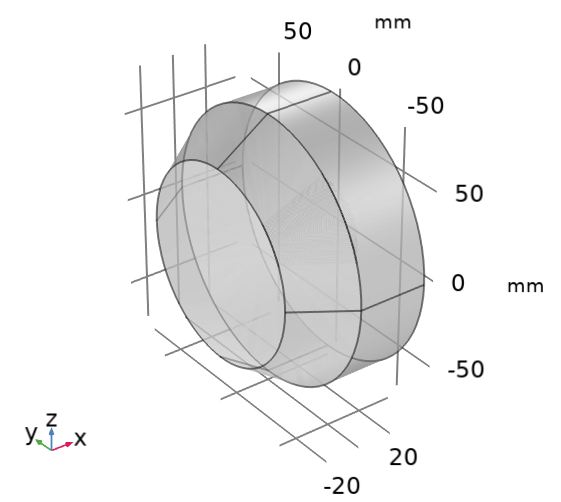
\includegraphics{../fig/fig_ConvNatComsol/Comsol_SimplifiedModel_Geometry5.png}
    \caption{Géométrie du modèle simplifié du régénérateur et de la cavité d'adaptation d'impédance.}
    \label{fig:Comsol_ModeleSimplifie_Geometrie}
\end{figure}

\subsection{Volume d'adaptation d'impédance}



\subsection{Régénérateur}
Le nombre de Rayleigh dans un matériau poreux dépend de sa perméabilité. Il est assez difficile de la calculer car il faut connaître la vitesse d'écoulement et la différence de pression de part et d'autre du domaine étudié. Le régénérateur est modélisé dans Comsol pour extraire ses paramètres hydrauliques et calculer les nombres adimensionnels déjà présentés.

De plus, cette simulation vise à vérifier l'hypothèse de superposition des effets thermiques. En effet, la distribution de température du côté de l'échangeur froid dans le cas de l'orientation `\texttt{H1}' laisse à penser que la température froide et constante sur la section provoqué par l'effet thermoacoustique, la conduction thermique dans le noyau qui provoque une différence de température entre le centre du noyau et sa périphérie, et la convection naturelle qui apporte un gradient de température selon la direction verticale se combinent.

\section{Modèle temporel} \label{chap:ModeleTemporel}
Un modèle temporel du régime transitoire de la distribution axiale de température dans le noyau thermoacoustique est créé pour approcher le réfrigérateur \textsc{Tacot} d'après le modèle 1D développé par Lotton \textit{et al.} pour un réfrigérateur à ondes stationnaires \cite{lotton_transient_2009}. Ce modèle calcule le bilan de chaleur au sein du régénérateur en faisant intervenir les flux de chaleur thermoacoustique $Q_{\sf TA}$, de conduction thermique $Q_{\sf cond}$, de frottement visqueux $Q_{\sf visq}$, et de pertes latéral au travers des parois de la cavité $Q_{\sf lat}$ dans chaque volume élémentaire $S_{\sf reg} \deriv x$ du régénérateur discrétisé. Pour compenser les écarts entre les prévisions du modèle et les mesures, un flux de chaleur $Q_{\sf vort}$ estimé empiriquement est également pris en compte dans les conditions aux frontières sur l'axe du noyau. Ce flux est supposé lié aux effets de bord du noyau tels que la vorticité, les pertes de charges ou les effets entropiques. Ce modèle 2D prend en compte les conditions au limites suivantes : 



%\begin{comment}
Le modèle a pour but de calculer les transferts thermiques dans le régénérateur pour n'importe quel champ acoustique. Aussi, l'expression des quantités oscillantes dans le noyau peut-être donnée par un produit de matrices de transfert élémentaires de l'équation~\eqref{eq:TMatrix_prod_TppTuu}. Dans le cas d'un régénérateur compact du point de vue acoustique, les coefficients de cette matrice de transfert sont donnés par

\begin{subequations}
	\begin{multicols}{2}
	\noindent
	\begin{align}
		T_{pp}^{(n)} &= 1, \label{eq:TMatrix_Tpp_regen}\\
		T_{pu}^{(n)} &= -\frac{i \omega \rho}{\Phi S (1-f_\nu)}\deriv x, \label{eq:TMatrix_Tpu_regen}
		\end{align}
		\begin{align}
		T_{up}^{(n)} &= -\frac{i \omega \Phi S}{\gamma P_0} \deriv x, \label{eq:TMatrix_Tup_regen}\\
		T_{uu}^{(n)} &= 1. \label{eq:TMatrix_Tuu_regen}
	\end{align}
	\end{multicols}
	\label{eq:TMatrix_regen}
\end{subequations}

\subsection{Flux thermiques}
Ensuite, les flux thermiques sont également pour la plupart différents dans le cas d'un réfrigérateur contenant un régénérateur à la place d'un \textit{stack}, et sont définis dans les équations \eqref{eq:FluxTA_Lotton_Regen} à \eqref{eq:FluxLat_Lotton} accompagnées de la figure~\ref{fig:Schema_FluxThermiquesNoyau_Gaelle} pour les illustrer au sein du régénérateur.

\begin{figure}[!ht]
    \centering
    \external{fig_Schema_FluxThermiquesNoyau_Gaelle}
%    \externalremake
    \begin{tikzpicture}%[yscale=3]
	\def\Lreg{6cm};
	\def\Ryreg{4cm};
	\def\Rxreg{1cm};%{\Ryreg/3};
	\def\CHXnorth{0,\Ryreg};
	\def\CHXsouth{0,-\Ryreg};
	\def\AHXnorth{\Lreg,\Ryreg};
	\def\AHXsouth{\Lreg,-\Ryreg};
	

	


% --------------------------------------------------- Flux thermiques
%\fill[MatlabBlue,opacity=.5] (\CHXnorth) arc [start angle=90, end angle=270, x radius=\Rxreg, y radius=\Ryreg] -- cycle; % Face gauche (fond)
%\draw[very thick] (\CHXnorth) arc [start angle=90, end angle=270, x radius=\Rxreg, y radius=\Ryreg]; % Face gauche (contour)

\filldraw[fill=MatlabBlue, fill opacity=.5, draw=black,very thick] (\CHXnorth) rectangle (\AHXsouth);

%%% Q_vort
\foreach \y in {-.5,0,.5}{
\draw[arw,->,draw=MatlabPurple,line width=1mm] (-.1*\Rxreg,{(\y+.02)*\Ryreg}) -- ++(-\Rxreg,0) arc (-90:-360:.35);
\draw[arw,->,draw=MatlabPurple,line width=1mm] (-.1*\Rxreg,{(\y-.02)*\Ryreg}) -- ++(-\Rxreg,0) arc (90:360:.35);
\draw[arw,->,draw=MatlabPurple,line width=1mm] (\Lreg+.1*\Rxreg,{(\y+.02)*\Ryreg}) -- ++(\Rxreg,0) arc (-90:180:.35);
\draw[arw,->,draw=MatlabPurple,line width=1mm] (\Lreg+.1*\Rxreg,{(\y-.02)*\Ryreg}) -- ++(\Rxreg,0) arc (90:-180:.35);}

\draw (-1.2*\Rxreg,-.5*\Ryreg) node[left]{$\left.Q_{\sf vort}\right|_{x=0}$};
\draw (\Lreg+1.2*\Rxreg,.5*\Ryreg) node[right]{$\left.Q_{\sf vort}\right|_{x=L_{\sf reg}}$};

% --------------------------------------------------- Fond de schéma

\draw[dotted, ->, very thick] ({-3.5*\Rxreg},-\Ryreg) -- ({\Lreg+3.5*\Rxreg},-\Ryreg) node [right] {$\mathbf e_x$}; % axe x
%\fill[MatlabBlue,opacity=.5] (\CHXnorth) arc [start angle=90, end angle=-90, x radius=\Rxreg, y radius=\Ryreg] -- cycle; % bord gauche (moitié droite pour que l'axe x rentre "dans le noyau")
\draw[dotted, ->, very thick] ($(\CHXsouth)+(0,-.3*\Ryreg)$) -- ($(\CHXnorth)+(0,.3*\Ryreg)$) node [above] {$\mathbf e_r$}; % axe r

%\draw[dashed, very thick] (\AHXnorth) arc [start angle=90, end angle=270, x radius=\Rxreg, y radius=\Ryreg]; % paroi gauche arrière pointillée
%\filldraw[fill=MatlabBlue, fill opacity=.5, draw=black,very thick] (\CHXnorth) arc [start angle=90, end angle=-90, x radius=\Rxreg, y radius=\Ryreg] -- (\AHXsouth) arc [start angle=-90, end angle=90, x radius=\Rxreg, y radius=\Ryreg] --cycle; % Paroi du cylindre


% --------------------------------------------------- Dimensions
\draw (\CHXnorth) node [above right] {\begin{tabular}{ll}\'Echangeur \\  froid\end{tabular}};
\draw (\AHXnorth) node [above left] {\begin{tabular}{rr}\'Echangeur \\ ambiant \end{tabular}  };

\draw (0,-\Ryreg) node[below left] {0};
\draw (\Lreg,-\Ryreg) node{|} node[below left] {$L_{\sf reg}$};
\draw (\CHXnorth) -- ++(-.5cm,0) node[left] {$2 R_{\sf reg}$};

%%% Q_TA
\draw[arw,->,draw=MatlabBlue] ({.25*\Lreg},0) -- ++(.33*\Lreg,0) node[right] {$Q_{TA}$} node(MidQTA)[midway]{};
%
%\draw[arw,<-,draw=MatlabBlue] ($(\CHXsouth)+(-1mm,-1mm)$) -- ++(-120:.33*\Lreg)node[pos=.75, left]{$Q_{TA}(0)$};
%\draw[arw,->,draw=MatlabBlue] ($(\AHXsouth)+(1mm,-1mm)$) -- ++(-60:.33*\Lreg)node[pos=.25, right]{$Q_{TA}(L_{\sf reg})$};

%%% Q_cond
\draw[arw,->,draw=MatlabOrange] ({.75*\Lreg},.15*\Ryreg)  -- ++(-.33*\Lreg,0) node[left] {$Q_{\sf cond}^{(x)}$} node(MidCondx1)[midway]{};
\draw[arw,->,draw=MatlabOrange] ({.75*\Lreg},-.15*\Ryreg)  -- ++(-.33*\Lreg,0) node(MidCondx2)[midway]{} node[left] {$Q_{\sf cond}^{(x)}$};

\draw[arw,->,draw=MatlabYellow] ({.25*\Lreg},.3*\Ryreg)  -- ++(0,.33*\Lreg) node[above] {$Q_{\sf cond}^{(r)}$} node(MidCondr1)[midway]{};
\draw[arw,->,draw=MatlabYellow] ({.75*\Lreg},-.3*\Ryreg)  -- ++(0,-.33*\Lreg) node[below] {$Q_{\sf cond}^{(r)}$} node(MidCondr2)[midway]{};

%%% Q_visq
\draw[arw,<->,draw=PythonGreen] ($(MidCondr1 -| MidCondx1)+(-.33*\Lreg/2,0)$)  -- ++(.33*\Lreg,0) node[midway,above]{$Q_{\sf visq}$};
\draw[arw,<->,draw=PythonGreen] ($(MidCondr2 -| MidQTA)+(-.33*\Lreg/2,0)$)  -- ++(.33*\Lreg,0) node[midway,below]{$Q_{\sf visq}$};


%%% Q_lat
\draw[->,line width=1mm,decorate,decoration={snake,amplitude=.4mm,segment length=2mm,post length=2mm},red] (.5*\Lreg,1.1*\Ryreg) -- ++(0,1cm) node [above] {$\left.h_r\right|_{r=2R_{\sf reg}}\theta$};
\draw[->,line width=1mm,decorate,decoration={snake,amplitude=.4mm,segment length=2mm,post length=2mm},red] (.5*\Lreg,-1.1*\Ryreg) -- ++(0,-1cm) node [below] {$\left.h_r\right|_{r=0}\theta$};

%\draw[red] (.5*\Lreg,1.1*\Ryreg) node{$T_{paroi}$}; 
%\draw[red, line width=1mm] ($(\CHXnorth)+(0,0)$) -- ($(\AHXnorth)+(0,0)$);
%\draw[red] (.5*\Lreg,-1.1*\Ryreg) node{$T_{paroi}$};
%\draw[red, line width=1mm] ($(\CHXsouth)+(0,0)$) -- ($(\AHXsouth)+(0,0)$);

\draw[->,line width=1mm,decorate,decoration={snake,amplitude=.4mm,segment length=2mm,post length=2mm},red] (-2*\Rxreg,0) -- ++(-1cm,0) node [midway, above] {$\left.h_x\right|_{x=0}\theta$};
\draw[->,line width=1mm,decorate,decoration={snake,amplitude=.4mm,segment length=2mm,post length=2mm},red] (\Lreg+2*\Rxreg,0) -- ++(1cm,0) node [midway, above] {$\left.h_x\right|_{x=L_{\sf reg}}\theta$};

%%% Q_HX
%\draw[arw,<-,draw=gray] ($(\CHXsouth)+(1mm,-1mm)$) -- ++(-60:.33*\Lreg)node[pos=.75, right]{$Q_f$};
%\draw[arw,->,draw=gray!50!black] ($(\AHXsouth)+(-1mm,-1mm)$) -- ++(-120:.33*\Lreg)node[pos=.25, left]{$Q_a$};
\draw[arw,<-,draw=gray] ($(\CHXsouth)+(0,-5mm)$) -- ++(0,-.33*\Lreg)node[pos=.75, right]{$Q_f$};
\draw[arw,->,draw=gray!50!black] ($(\AHXsouth)+(0,-5mm)$) -- ++(0,-.33*\Lreg)node[pos=.25, left]{$Q_a$};

\end{tikzpicture}
    \caption{Représentation schématique des flux thermiques considérés dans le modèle transitoire du régénérateur.}
    \label{fig:Schema_FluxThermiquesNoyau_Gaelle}
\end{figure}

\begin{enumerate}[label=\textbf{(\roman*)}]
\item Tout d'abord, le flux thermoacoustique 1D est calculé avec l'équation~\eqref{eq:FluxTA_swift} développée par Swift \cite{swift_thermoacoustics_2017}

\begin{multline}
	Q_{TA} = \underbrace{ -\frac12~\RE\left[ \frac{ f_\kappa-f_\nu^* }{ (1+\mathrm{Pr})(1-f_\nu^*) } pu^* \right] }_{q_{TA}(x)} \\ 
	+ \overbrace{ \frac12 \frac{\rho_0 C_p}{\Phi S}~\IM\left[ \frac{f_\kappa + \mathrm{Pr} f_\nu^*}{(1-\mathrm{Pr}^2)|1-f_\nu|^2} \right] |u|^2 }^{k_{TA}(x)}\partial_x \theta(r,x;t),
\label{eq:FluxTA_Lotton_Regen}
\end{multline}
où $\theta(r,x;t) = T_0(r,x;t)-T_\infty$ est l'écart de la température locale à la température initiale. Pour la suite du document, cet écart de température sera simplement écrit $\theta$, sans la dépendance spatio-temporelle. Il est important de remarquer la partie réelle de ce flux thermique, notée $q_{TA}$, qui ne dépend que du champ acoustique, et la partie imaginaire $k_{TA}$ qui dépend du gradient de température le long du stack et qui peut être vu comme un terme de conduction induite par l'effet thermoacoustique.

\item Ensuite, la conduction dans le régénérateur est prise en compte dans les directions $\textbf e_x$ et $\textbf{e}_r$ du régénérateur avec l'équation exprimée en coordonnées cylindriques par

%\begin{equation}
%	Q_{\sf cond} = -\begin{pmatrix}
%	k_x\\
%	k_r\\
%	k_\alpha
%	\end{pmatrix} \cdot \nabla \theta,
%	\label{eq:FluxCond_Lotton}
%\end{equation}

\begin{equation}
	\left\{ \begin{aligned}
		Q_{\sf cond}^{(x)} &= -k_x \partial_x T\\
		Q_{\sf cond}^{(r)} &= -k_r \partial_r T \echaf{\text{ corriger expression avec gradient radial}}
	\end{aligned}\right.
	\label{eq:FluxCond_Lotton}
\end{equation}
avec les indices $x$ et $r$ dénotant respectivement les directions axiale et radiale où circulent les flux de conduction. La porosité influe sur la conductivité thermique apparente et $k_i~=~\Phi_i k_{g} + (1-\Phi_i)k_{s}$ ($i=x,r$). \echaf{En première aproximation, il est possible de considérer les valeurs de conductivité comme égales les unes aux autres. Cependant, c'est inexact car le long de l'axe $\mathbf e_x$ le milieu est constitué de l'empillement de tissus métalliques tandis que dans la direction $\mathbf e_r$ le flux de chaleur parcourt les fils qui forment le tissus en lui-même.}

%\begin{equation}
%Q_{\sf cond}^{(x)} = -k_x\partial_x\theta~\mathrm{\mathbf e_x},
%\label{eq:FluxCondx_Lotton}
%\end{equation}
%avec... 
%
%\begin{equation}
%Q_{\sf cond}^{(r)} = -k_r\partial_r\theta~\mathrm{\mathbf e_r},
%\label{eq:FluxCondr_Lotton}
%\end{equation}
%
%\begin{equation}
%Q_{\sf cond}^{(\alpha)} = -k_\alpha\partial_\alpha\theta~\mathrm{\mathbf e_\alpha},
%\label{eq:FluxCondalpha_Lotton}
%\end{equation}
%\textcolor{red}{Rassembler $Q_{cond}$ en 1 seul terme} avec ...

\item Les pertes visqueuses sont estimées avec l'équation

\begin{equation}
Q_{\sf visq} = \frac{1}{R_{\sf reg}^2} \int_{0}^{R_{\sf reg}} \frac{1}{\tau_0} \int_0^{\tau_0} \mu (\partial_r u)^2\ r \deriv r \deriv t.
\label{eq:FluxVisq_Lotton}
\end{equation}

En utilisant l'identité

\begin{equation*}
\frac{1}{T}\int_{0}^{\tau_0}\mu(\partial_r u)^2\deriv t = \frac12|\partial_r u|^2,
\end{equation*}
l'équation \eqref{eq:FluxVisq_Lotton} est réécrite comme

\begin{equation}
	Q_{\sf visq} = \frac{1}{2R_{\sf reg}^2} \int_{0}^{R_{\sf reg}} \mu |\partial_r u|^2\ r \deriv r
	\label{eq:FluxVisq_Lotton_IntegralTSimplifie}
\end{equation}

\echaf{poursuivre après simu}
dont l'intégrale sur la section de rayon $R_{\sf reg}$ est résolue par une méthode numérique.

\item Les effets de bords tels que les pertes de charges ou la vorticité sont pris en compte aux frontières du domaine grâce à des flux de chaleur $Q_{\sf vort}$ estimés empiriquement à $x=0$ et $x=L_{\sf reg}$.

\item Enfin, les pertes latérales sur la circonférence et aux extrémités du régénérateur sont prises en compte par

\begin{equation}
	\left\{ \begin{aligned}
		Q_{\sf lat}^{(x)} &= h_x \theta,\\
		Q_{\sf lat}^{(x)} &= h_x \theta,
	\end{aligned}\right.
\label{eq:FluxLat_Lotton}
\end{equation}
où $h_x$ et $h_r$ sont respectivement les coefficients d'échanges avec les extrémités à $x=0$ et $x=L_{\sf reg}$, et avec la paroi à $r = R_{\sf reg}$. Ils sont déterminés de façon empirique dans l'article.

%Alternativement, il est possible de prendre en compte les échanges de chaleur au bord et dans l'axe du noyau par un terme qui représente le flux de chaleur induit par les oscillations acoustiques noté $\psi_{ac}$ dans la thèse de Guédra \cite{guedra_etudes_2012} et défini par
%
%\begin{equation}
%	\psi_{ac}=\frac12 \rho_0 T_0 \RE[s v^*],
%	\label{eq:FluxChaleurAcou_Guedra}
%\end{equation}
%dont la moyenne sur la section s'écrit
%
%\begin{align}
%	\langle\psi_{ac}\rangle &= \RE[g]\mathcal I \IM[g]\mathcal J - k_{ac}\deriv_x T_0,	\label{eq:FluxChaleurAcou_Guedra_Moy}\\
%										&= \langle\psi_{ac,0}\rangle
%\end{align}

\end{enumerate} 

\subsection{Conditions aux limites}
\begin{enumerate}[label=\textbf{(\roman*)}]
\item \echaf{Condition de température sur le canister}


\begin{figure}[!ht]
    \centering
    \external{fig_TemperatureCanisterConditionLimite}
    %\externalremake
    \begin{tikzpicture}
	\def\lREG{3.9cm};
	\def\eCAN{5mm};
	\def\eWALL{13pt};
	\def\eFB{6mm};
	
	\fill[gray] (0,0) node(O){} rectangle (\lREG,-\eCAN);
	\fill[top color=gray,bottom color=white](0,-\eCAN) node(eCAN){} rectangle (\lREG,-2*\eCAN);
	
	\fill[right color=black!25,left color=white] ($(O)+(0,\eWALL)$) node(eWALL){} rectangle (-\lREG/4,0);
	\fill[black!25] (O) rectangle (\lREG,\eWALL) node[midway]{$k_{\sf acier}$};
	\fill[right color=white,left color=black!25] ($(O)+(\lREG,0)$) rectangle ++(\lREG/4,\eWALL);
	
	\fill[blue!25!white] ($(O)+(0,\eWALL+\eFB)$) node(eFB){} rectangle ++(\lREG,-\eFB);
	\fill[right color=blue!25!white,left color=white] (eFB) rectangle ++(-\lREG/4,-\eFB);
	\fill[right color=white,left color=blue!25!white] ($(eFB)+(\lREG,0)$) rectangle ++(\lREG/4,-\eFB);
	\fill[top color=white,bottom color=blue!25!white] (eFB) rectangle ++(\lREG,.5*\eFB);
	\shade[upper left=white,upper right=white,
         lower left=white,lower right=blue!25!white] (eFB) rectangle ++(-\lREG/4,.5*\eFB);
	\shade[upper left=white,upper right=white,
         lower left=blue!25!white,lower right=white] ($(eFB)+(\lREG,0)$) rectangle ++(\lREG/4,.5*\eFB);
	\draw[->,line width=.5mm,decorate,decoration={snake,amplitude=.4mm,segment length=2mm,post length=2mm},blue!75!white] ($(eWALL)+(\lREG/2,0)$) -- ++(0,\eFB) node[midway,right,blue!75!white]{$h_{\sf conv}$};
	
	
	
	\draw[->] ($(eFB)+(0,\eFB)$) -- ($(eCAN)+(0,-2.1*\eCAN)$) node[left]{$-\mathbf{e}_r$};
	\draw[->] (-1mm,0) node(lab){} -- (4*\lREG/3,0) node[above]{$\mathbf{e}_x$};
	
	\draw ($(eWALL) + (-\lREG/4,1.5*\eFB/2)$) node[left]{Canal de rétroaction};
	\draw ($(O) + (-\lREG/4,\eWALL/2)$) node[left]{Tube contenant le noyau};
	\draw (eWALL) node[left]{$e_{\sf wall}$};
	\draw (O) node[left]{0};
	\draw[line width=.5mm,dashed] (eCAN.base) node[left]{$e_{\sf can}$} -- ++(\lREG,0);
\end{tikzpicture}
    \caption{Géométrie équivalente pour établir la condition de température à la frontière $r=R_{\sf reg}$.}
    \label{fig:TemperatureCanisterConditionLimite}
\end{figure}

\item \echaf{Flux de chaleur apportés ou retirés par les échangeurs}

$Q=\epsilon Q_i$ avec 
\begin{equation}
	\epsilon = \frac{k_s k_{sfrac} (1-\Phi)S_{\sf reg}}{k_s k_{sfrac} (1-\Phi)S_{\sf reg} + k_{\sf can} S_{\sf can}}
\end{equation}
et $k_{sfrac}$ le facteur de dégradation de conductivité \cite{lewis_measurement_1998}

\end{enumerate}

\subsection{Bilan thermique}

Ces flux de chaleurs sont reportés dans l'équation modifiée du bilan de chaleur qui s'écrit

%\begin{equation}
%[\Phi\rho_0 C_p + (1-\Phi)\rho_s C_s]\partial_t \theta = - \nabla \cdot (Q_{TA} + Q_{\sf cond}) + Q_{\sf visq},
%\label{eq:BilanChaleur_LottonPoignand}
%\end{equation}
%ce qui donne après développement de l'opérateur divergence en coordonnées cylindrique,

\begin{equation}
[\Phi\rho_0 C_p + (1-\Phi)\rho_s C_s]\ \partial_t \theta = - \partial_x Q_{TA} - \partial_x Q_{\sf cond}^{(x)} - \frac{1}{r}\partial_r[r Q_{\sf cond}^{(r)}] + Q_{\sf visq}.
\label{eq:BilanChaleur_LottonPoignand_ApDvptCylin}
\end{equation}

Le premier membre désigne la variation d'énergie interne suite à la variation de température, et le second membre, l'expression des flux thermiques dans chaque volume élémentaire. D'une part, les flux thermoacoustiques et de conduction sont \og de passage \fg{} au travers de ce volume, et c'est seulement dans le cas d'une divergence non nulle que la température y évolue. D'autre part, les effets visqueux se produisent dans chaque volume, il sont donc source de chaleur et doivent être pris en compte tels quels. Ceci dit, le régénérateur est supposé axisymétrique, ce qui permet de considérer les composantes azimuthales $\nabla_\alpha \cdot Q_{TA}$ et $\nabla_\alpha \cdot Q_{\sf cond}$ comme nulles.

Le problème décrit par l'équation~\ref{eq:BilanChaleur_LottonPoignand_ApDvptCylin} est conditionné aux frontières en $x=0$, $x=L_{\sf reg}$ et $r=R_{\sf reg}$ pour respecter la conservation d'énergie. Ces conditions se traduisent par le système d'équations

\begin{subequations}
	\begin{align}
		Q_{\sf cond}^{(x)} + Q_f + Q_{\sf vort}(0) &= Q_{TA}(0) + h_x(0)\theta,\quad &x=0,\ r \in [0,R_{\sf reg}], t>0 \label{eq:CondFront_x_0Froid}\\%
		Q_{TA}(L_{reg}) + Q_{\sf vort}(L_{reg})  &= Q_{\sf cond}^{(x)} + Q_a + h_x(L_{\sf reg})\theta, \quad &x=L_{\sf reg},\ r \in [0,R_{\sf reg}], t>0 \label{eq:CondFront_x_LregAmb}\\%
		Q_{\sf cond}^{(r)} &= h_r(R_{\sf reg})\theta, \quad &r=R_{\sf reg},\ x \in [0,L_{\sf reg}], t>0 \label{eq:CondFront_r_ra}
	\end{align}%
	\label{eq:CondFront}%
\end{subequations}
où $Q_f$ et $Q_a$ sont les flux de chaleur retirés à l'échangeur froid d'une part et apporté à l'échangeur ambiant d'autre part. Ce système signifie que pour chaque frontière, la somme des flux entrant dans l'interface et des sources thermiques est égale aux flux qui en sortent. Il reste à introduire la distribution de température à $t=0$ notée $\theta_0(x,r)$ comme condition initiale, qui se présente comme

\begin{equation}
	\theta(x,r,t=0) = \theta_0(x,r).
	\label{eq:CondInit}
\end{equation}

Le report des flux de chaleurs des équations~\eqref{eq:FluxTA_Lotton_Regen} à \eqref{eq:FluxLat_Lotton} dans l'équation du problème~\eqref{eq:BilanChaleur_LottonPoignand_ApDvptCylin}, dans les conditions aux frontières~\eqref{eq:CondFront} et dans la condition initiale~\eqref{eq:CondInit} permet de poser le problème tel que

\begin{equation}
	toto
	\label{eq:ProbTransitoire_ApDvpt}
\end{equation}

\subsection{Méthode des transformations intégrales}

La résolution de l'équation~\eqref{eq:BilanChaleur_LottonPoignand_ApDvptCylin} qui comporte des termes sources requiert l'usage de la méthode des transformations intégrales après réécriture des équations du système sous la forme d'un problème homogène équivalent \cite{ozisik_heat_1993}. Les équations s'écrivent alors

\begin{subequations}
	\begin{align}
		\echaf{Systeme\ ici},\label{eq:1_LottonPoignand}\\
		\echaf{Systeme\ ici},\label{eq:2_LottonPoignand}
	\end{align}
	\label{eq:SystemeEq_LottonPoignand}
\end{subequations}
avec les changements de variables suivants

\begin{itemize} \color{red}
	\item 1
	\item 2.
\end{itemize}

%\end{comment}

